\documentclass[12pt]{article}
\usepackage[english]{babel}
\usepackage{float}
\usepackage[margin=1in]{geometry}
\usepackage{graphicx}
%\usepackage[toc,page]{appendix}
\graphicspath{ {./img/} }
\newcommand{\rpm}{\raisebox{.2ex}{$\scriptstyle\pm$}} 
\usepackage{listings}
\usepackage{xcolor}
\usepackage{indentfirst}
\usepackage{caption}
\usepackage[final]{pdfpages}
\usepackage{amsmath}
\usepackage[normalem]{ulem}



\begin{document}

\title{Joe Phaneuf \\ Computer Vision 16-720 Spring 2018 Homework 6 \\ Apr. 28 2018 }
\date{}
\author{}
\maketitle

\newpage


%\stepcounter{section}
%%%%%%%%%%%%%%%%%%%%%%%%%%%%%%%%%%%%%%%%%%%%%%%%%%%%%%%%%%%%%%%%%%%%%%%%%%%%%%%%
%%%%%%%%%%%%%%%%%%%%%%%%%%%%%%%%%%%%%%%%%%%%%%%%%%%%%%%%%%%%%%%%%%%%%%%%%%%%%%%%
\section{Q1}
\subsection{Q1.1}
For Lucas-Kanade Tracking, we aim to iteratively compute an optimal image transformation. At each iteration, the optimal change in transform parameters $\Delta p$ is found by linearization as seen in equation \ref{eq:iteration}.

\begin{equation}
\label{eq:iteration}
\Delta p ^{*} = argmin_{\Delta p} \sum_{x}
\begin{bmatrix}
\nabla I \frac { \partial W } { \partial p } \Delta p - \{ T ( x ) - I ( W ( x ; p ) ) \}
\end{bmatrix}^{2}
\end{equation}

Where $I$ is a target image, $\nabla I$ is the image gradient, $W$ is the image transformation function, $\frac{ \partial W } { \partial p }$ is the Jacobian representing the change in pixel position with respect to transform parameters $p$, and $T$ is the template image.

Equation \ref{eq:iteration} can be set up in normal equation form $argmin_{\Delta p} || A \Delta p - b ||_{2}^{2}$ where $A$ and $b$ are:
\begin{equation}
\label{eq:A}
A =
\nabla I \frac { \partial W } { \partial p }
\end{equation}
\begin{equation}
\label{eq:A}
b = T ( x ) - I ( W ( x ; p ) )
\end{equation}

This method banks on a few assumptions to obtain a unique $\Delta p$. First, $A^{T} A$ must be invertible for a solution to be obtained. Also, the eigen values of $A^{T} A$, $\lambda_{1}$ and $\lambda_{2}$, must be sufficiently large, and well conditioned ( $\lambda_{1}$ not significantly larger than $\lambda_{2}$ ). In human terms, this corresponds to the existence of corners in the the image, which allows for tracking.

\stepcounter{subsection}
\subsection{Q1.3}

Figure \ref{fig:suv} shows the resulting tracking bounding box following an SUV using the Lucas Kanade Inverse Compositional Algorithm. The SUV is tracked reasonably well across the image sequence.

\begin{figure}[H]
\centering
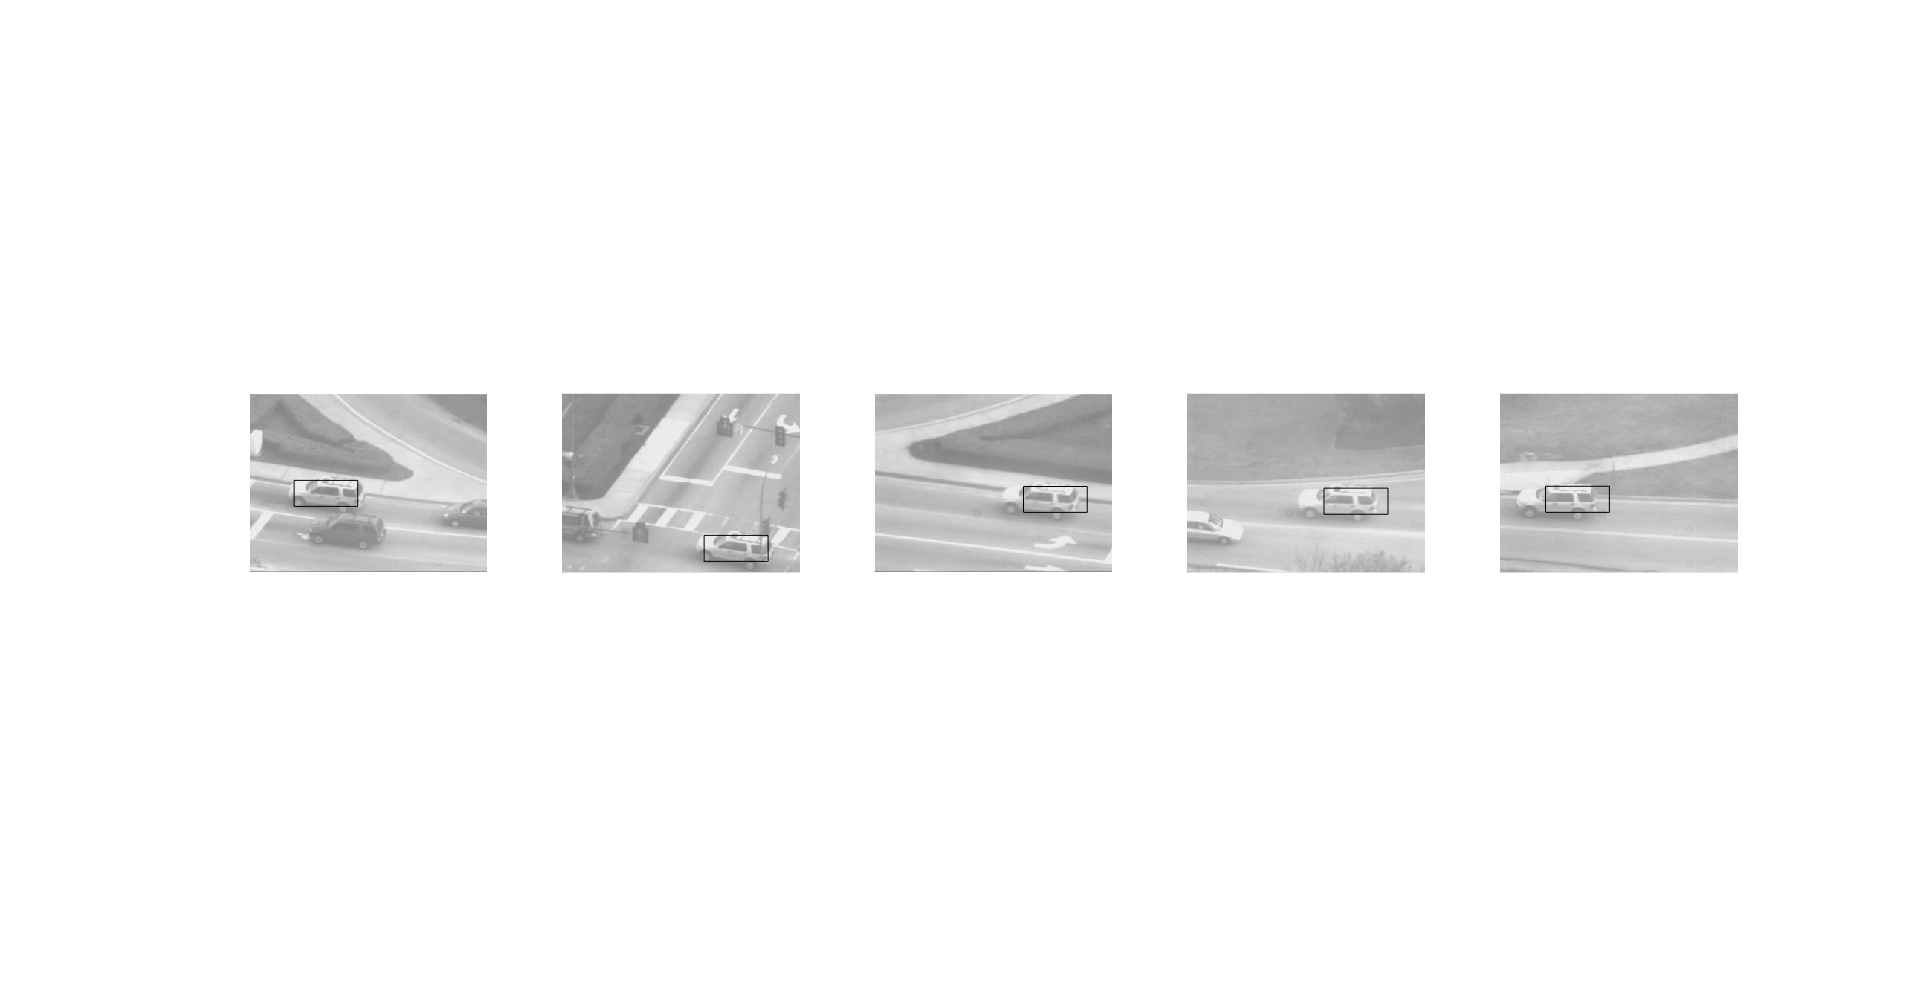
\includegraphics[page=1,width=1.0\textwidth]{q13_suv}
\caption{ SUV tracked at frames 1 , 100 , 200 , 300 , 400 } 
\label{fig:suv}
\end{figure}   

Figure \ref{fig:usvessel} shows the resulting bounding box following an SUV using the same algorithm tracking a beating heart vessel. This algorithm has more trouble tracking the vessel, which has fewer trackable  features than the SUV.

\begin{figure}[H]
\centering
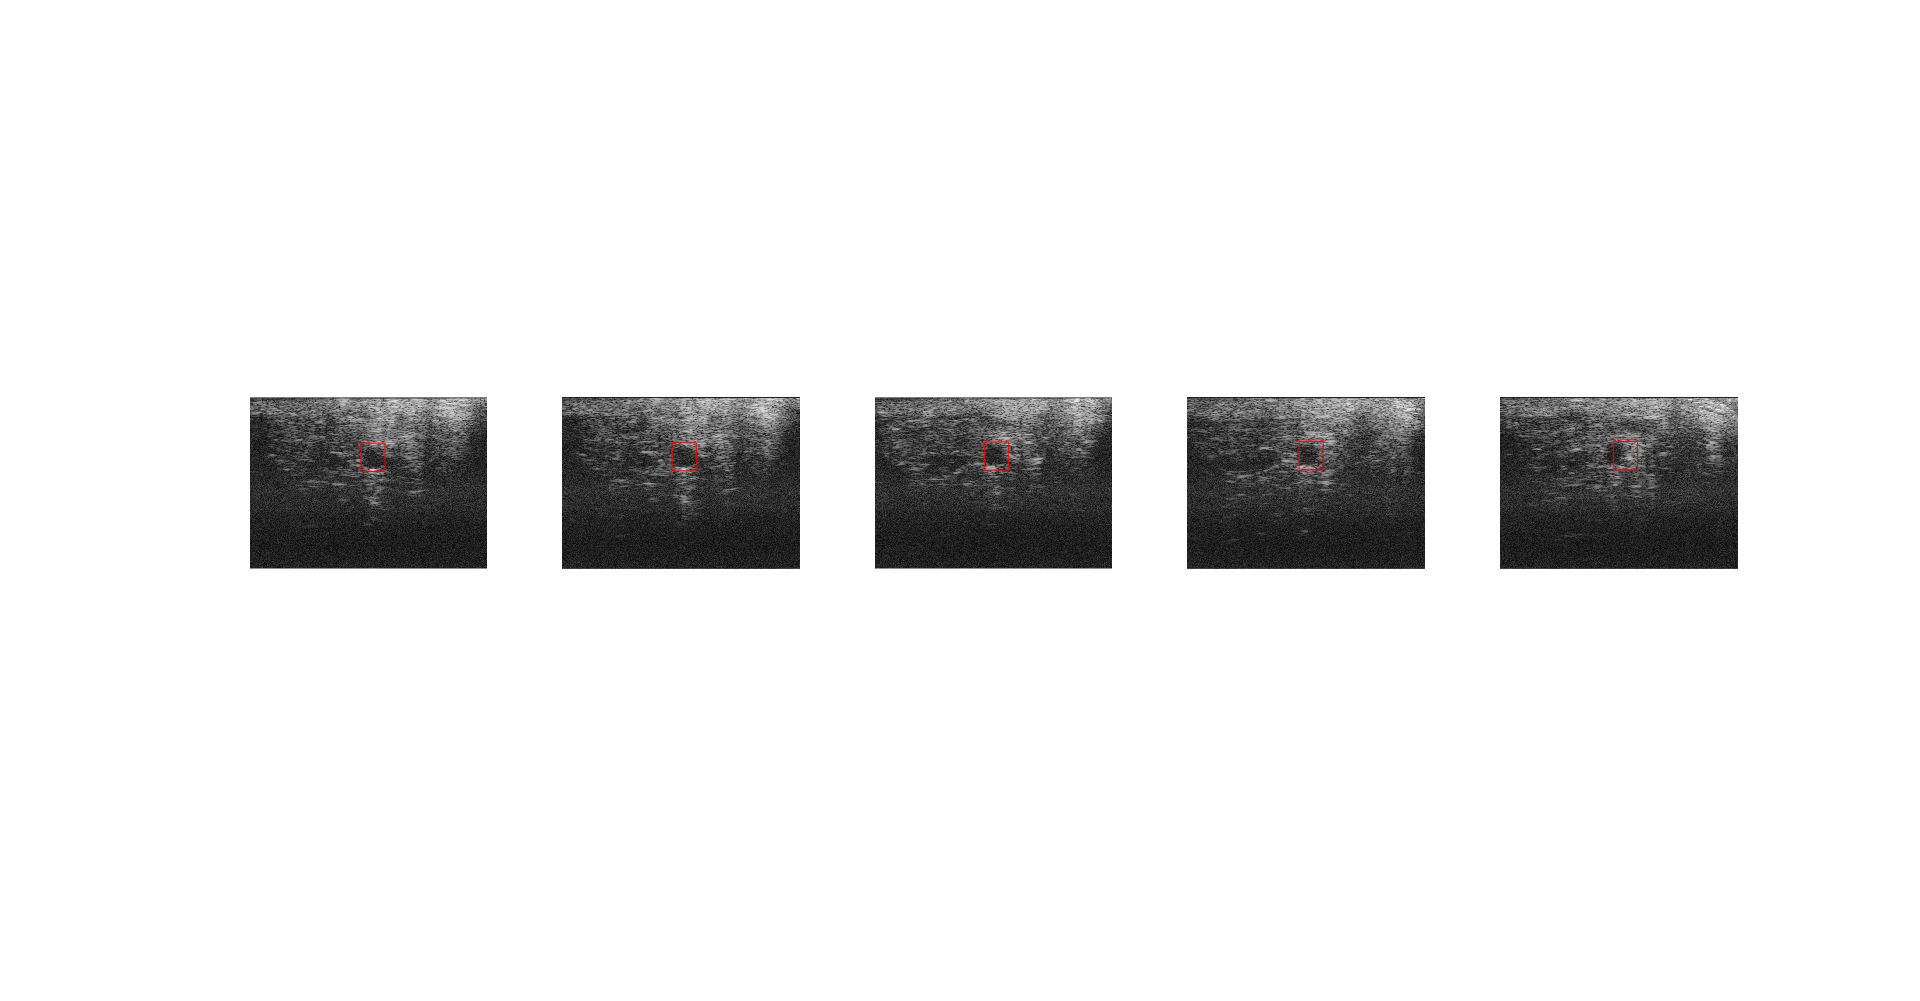
\includegraphics[page=1,width=1.0\textwidth]{q13_us}
\caption{ Beating vessel tracked at frames 5 , 25 , 50 , 75 , 100 } 
\label{fig:usvessel}
\end{figure}   


\section{Q2}
\subsection{Q2.1}
The appearance variation of a new frame can be approximated as a linear combination of the previous frame with a set of bases weighted by $\textbf{w}$ ( equation \ref{eq:w} ), with eacth weight $w_{k}$ is found using equation \ref{eq:wk}.

\begin{equation}
\label{eq:w}
\textbf { w } =
\begin{bmatrix}
w_{k}, ... , w_{K}
\end{bmatrix}
\end{equation}

\begin{equation}
\label{eq:wk}
w_{k}  = 
\sum_{x} B_{k} ( x )
\begin {bmatrix}
I ( W ( x ; p ) ) - T ( x )
\end {bmatrix}
\end{equation}

\stepcounter{subsection}
\subsection{Q2.3}
Figure \ref{fig:sylv} shows Sylvester the cat's head being tracked by both the Lucas Kanade Inverse Compositional algorithm ( red  bounding box ), as well as the Appearance Basis variant(blue bounding box) at frames 1, 200, 300, 350 and 400. Both algorithms track Sylvester's head well.
\begin{figure}[H]
\centering
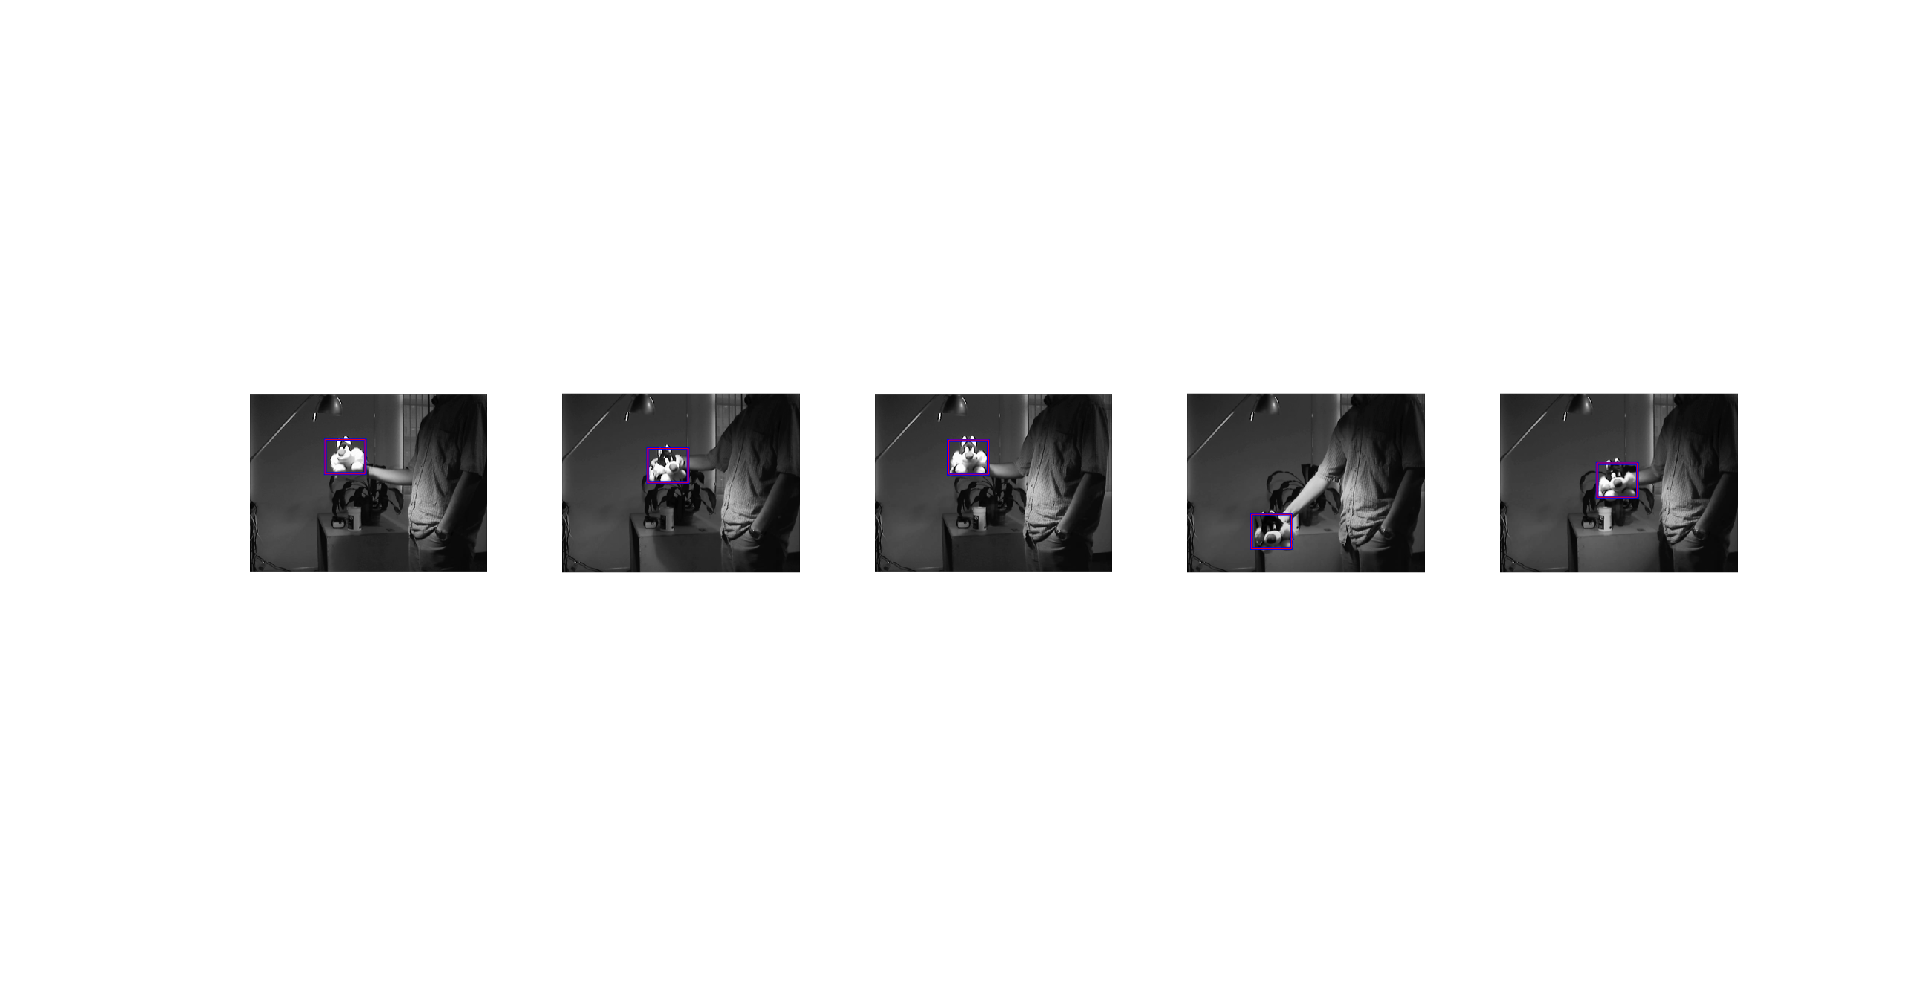
\includegraphics[page=1,width=1.0\textwidth]{q23}
\caption{ Sylvesters' head tracking: inverse compositional is red , basis is blue } 
\label{fig:sylv}
\end{figure}   

\section{Q3}
\stepcounter{subsection}
\stepcounter{subsection}
\subsection{Q3.3}
Figure \ref{fig:aerial} shows the results of overhead tracking of cars ( if you thought they were watching you, you were right ) with dominant motion estimation at frames 30 , 60 , 90 and 120.
\begin{figure}[H]
\centering
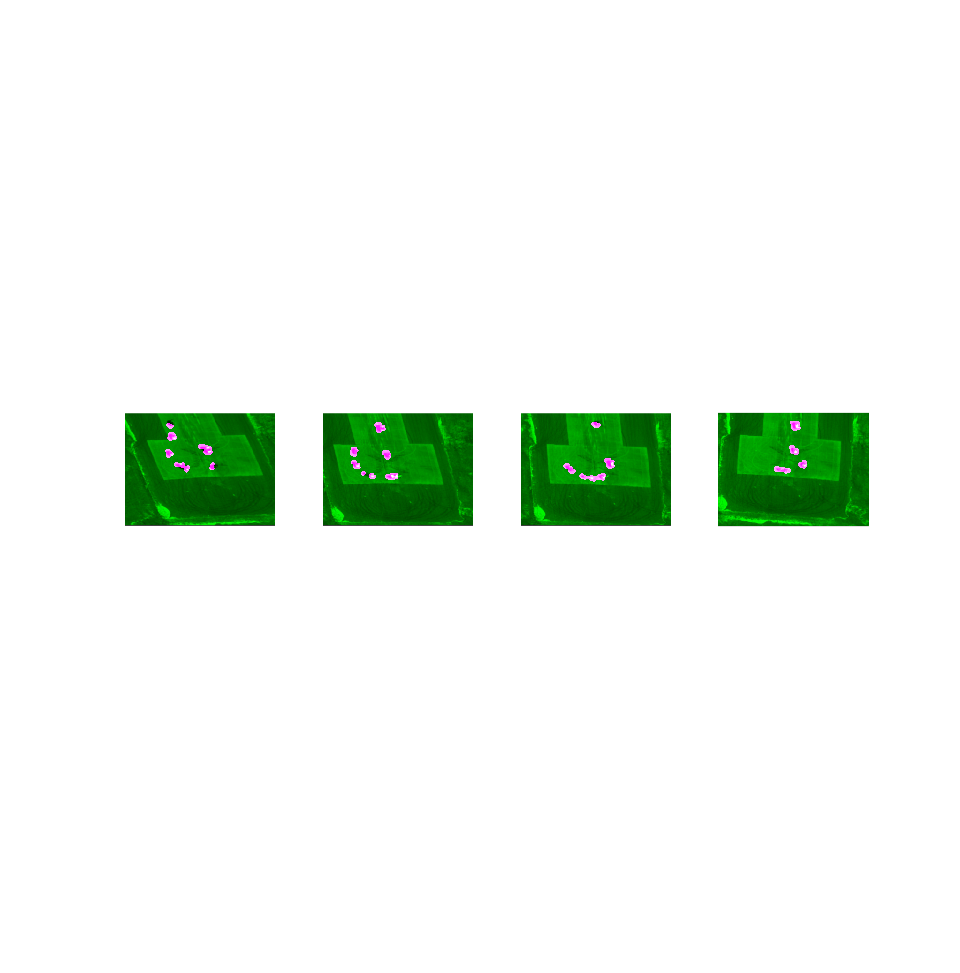
\includegraphics[page=1,width=1.0\textwidth]{q33_cars}
\caption{ Overhead car tracking at frames 30 , 60 , 90 ,120 }
\label{fig:aerial}
\end{figure}   


Figure \ref {fig:domvessel} shows the results of tracking a beating heart using dominant motion tracking, while adding an additonal masking layer by selecting from bounding boxes found in section 1. Results are shown at frames 5 , 25 , 50 , 75 , 100.
\begin{figure}[H]
\centering
\includegraphics[page=1,width=1.0\textwidth]{q33_vessel}
\caption{ Beating vessel tracked and masked at frames 5 , 25 , 50 , 75 , 100 } 
\label{fig:domvessel}
\end{figure}   



\end{document}
